\documentclass[11pt,a4paper]{article}

\usepackage[margin=2.2cm]{geometry}
\usepackage{amsmath,amssymb,amsfonts}
\usepackage{booktabs}
\usepackage{tikz}
\usetikzlibrary{positioning,arrows.meta,calc}
\usepackage[ruled,vlined,linesnumbered]{algorithm2e}
\usepackage{hyperref}
\usepackage{enumitem}
\usepackage{xcolor}
\usepackage{array}
\usepackage{multirow}

\hypersetup{colorlinks=true,linkcolor=blue,citecolor=blue,urlcolor=blue}

\newcommand{\R}{\mathbb{R}}
\newcommand{\concat}{\,\|\,}
\newcommand{\bU}{\mathbf{U}}
\newcommand{\bV}{\mathbf{V}}
\newcommand{\emb}[1]{\mathbf{e}_{#1}}
\newcommand{\noinf}{\mathbf{e}_{\varnothing}}
\newcommand{\calL}{\textsc{CalcLeft}}
\newcommand{\calR}{\textsc{CalcRight}}
\newcommand{\calP}{\textsc{CalcParent}}

\title{Neural Computational Graph Decoder for BEMAC:\\A Complete Worked Example with $N=4$}
\author{Polar Codes MAC Project}
\date{}

\begin{document}
\maketitle
\tableofcontents
\newpage

%=============================================================================
\section{Problem Setup}
\label{sec:setup}
%=============================================================================

We decode a two-user Binary Erasure MAC (BEMAC) polar code with block length $N=4$, $n=\log_2 N = 2$, using the Neural Computational Graph (NCG) decoder with \emph{pure neural} CalcParent (GRU-gated residual).

\subsection{Channel Model}

The BEMAC channel has output $Z = X + Y$ (integer addition), where $X,Y \in \{0,1\}$ are the transmitted bits from users U and V respectively. The channel output alphabet is $\{0,1,2\}$.

\subsection{Decoding Path}

We use a Class B path with \texttt{path\_i}$\,= 2$:
\[
\mathbf{b} = [\underbrace{0,0}_{\text{U,U}},\;\underbrace{1,1,1,1}_{\text{V,V,V,V}},\;\underbrace{0,0}_{\text{U,U}}]
\]
where $0 = $ U-step and $1 = $ V-step.  The path has length $2N=8$.

\subsection{Message Bits and Encoding}

\textbf{Information bits:}
\[
\mathbf{u} = (u_1, u_2, u_3, u_4) = (1, 0, 1, 1), \qquad
\mathbf{v} = (v_1, v_2, v_3, v_4) = (0, 1, 1, 0).
\]

\textbf{Frozen sets:} We set $k_u = 2$ info bits for U (positions 3, 4 are info; positions 1, 2 are frozen to 0) and $k_v = 3$ info bits for V (positions 2, 3, 4 are info; position 1 is frozen to 0):
\[
\text{frozen}_u = \{1 \mapsto 0,\; 2 \mapsto 0\}, \qquad
\text{frozen}_v = \{1 \mapsto 0\}.
\]
With frozen constraints: $u_1 = 0, u_2 = 0$ (so we use $\mathbf{u} = (0, 0, 1, 1)$) and $v_1 = 0$ (so $\mathbf{v} = (0, 1, 1, 0)$).

\medskip
\textbf{Polar encoding} $\mathbf{x} = \mathbf{u} \cdot G_4$ applies bit-reversal then butterfly XOR.  The bit-reversal permutation for $n=2$ is $\pi = (0, 2, 1, 3)$.

\medskip
\noindent\textbf{User U:} $\mathbf{u} = (0, 0, 1, 1)$.
\begin{enumerate}[nosep]
\item Bit-reversal: $\mathbf{u}[\pi] = (u_0, u_2, u_1, u_3) = (0, 1, 0, 1)$.
\item Butterfly stage 1 ($\text{step}=1$): pairs $(0,1), (2,3)$; left $\oplus=$ right: $(0 \oplus 1,\; 1,\; 0 \oplus 1,\; 1) = (1, 1, 1, 1)$.
\item Butterfly stage 2 ($\text{step}=2$): pairs $(0,2), (1,3)$; left $\oplus=$ right: $(1 \oplus 1,\; 1 \oplus 1,\; 1,\; 1) = (0, 0, 1, 1)$.
\end{enumerate}
Result: $\mathbf{x} = (0, 0, 1, 1)$.

\medskip
\noindent\textbf{User V:} $\mathbf{v} = (0, 1, 1, 0)$.
\begin{enumerate}[nosep]
\item Bit-reversal: $(0, 1, 1, 0)$.
\item Stage 1: $(0 \oplus 1,\; 1,\; 1 \oplus 0,\; 0) = (1, 1, 1, 0)$.
\item Stage 2: $(1 \oplus 1,\; 1 \oplus 0,\; 1,\; 0) = (0, 1, 1, 0)$.
\end{enumerate}
Result: $\mathbf{y} = (0, 1, 1, 0)$.

\medskip
\textbf{Channel output:}
\[
\mathbf{z} = \mathbf{x} + \mathbf{y} = (0+0,\; 0+1,\; 1+1,\; 1+0) = (0, 1, 2, 1).
\]

\subsection{Neural Decoder Parameters}

Embedding dimension $d = 4$, channel vocabulary size $|\mathcal{Z}| = 3$.  The decoder has:
\begin{itemize}[nosep]
\item \texttt{EmbeddingZ}: lookup table $\{0,1,2\} \to \R^4$.
\item \texttt{CalcLeft}: MLP $\R^{12} \to \R^4$ (concatenation of parent-first, parent-second, right).
\item \texttt{CalcRight}: MLP $\R^{12} \to \R^4$ (concatenation of parent-first, parent-second, left).
\item \texttt{CalcParent}: GRU-gated residual module $\R^4 \times \R^4 \to \R^4$ (left, right $\to$ parent-first); plus linear $\R^4 \to \R^4$ for parent-second.
\item \texttt{Emb2Logits}: MLP $\R^4 \to \R^4$ (embedding $\to$ 4 joint logits for $(u,v) \in \{00,01,10,11\}$).
\item \texttt{Logits2Emb}: MLP $\R^4 \to \R^4$ (log-probabilities $\to$ embedding, used for leaf updates).
\item \texttt{no\_info\_emb}: learnable $\R^4$ vector for uninitialized edges.
\end{itemize}

%=============================================================================
\section{Binary Tree Structure}
\label{sec:tree}
%=============================================================================

\subsection{Tree Diagram}

For $N=4$, the computational graph is a complete binary tree with 3 internal vertices and 4 leaves:

\begin{center}
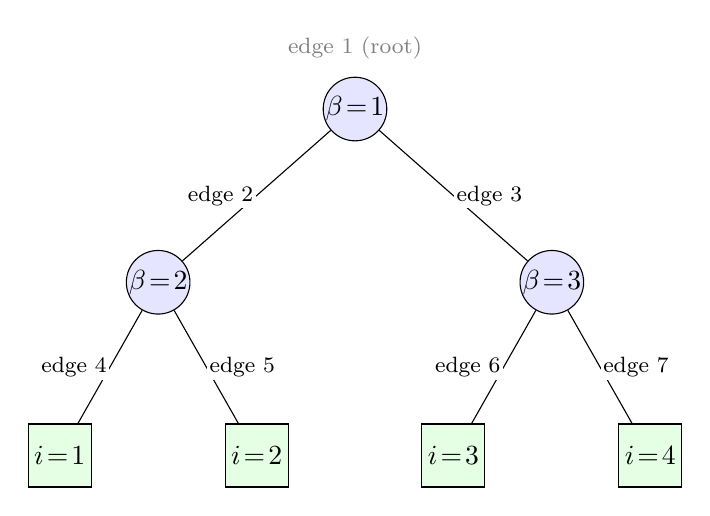
\begin{tikzpicture}[
    level 1/.style={sibling distance=5cm, level distance=2.2cm},
    level 2/.style={sibling distance=2.5cm, level distance=2.2cm},
    vertex/.style={circle, draw, minimum size=8mm, inner sep=0pt, fill=blue!10},
    edge label/.style={midway, fill=white, inner sep=1pt, font=\footnotesize},
    leaf/.style={rectangle, draw, minimum size=8mm, inner sep=1pt, fill=green!10}
]
\node[vertex] (v1) {$\beta\!=\!1$}
    child {
        node[vertex] (v2) {$\beta\!=\!2$}
        child {
            node[leaf] (l4) {$i\!=\!1$}
            edge from parent node[edge label, left] {edge 4}
        }
        child {
            node[leaf] (l5) {$i\!=\!2$}
            edge from parent node[edge label, right] {edge 5}
        }
        edge from parent node[edge label, left] {edge 2}
    }
    child {
        node[vertex] (v3) {$\beta\!=\!3$}
        child {
            node[leaf] (l6) {$i\!=\!3$}
            edge from parent node[edge label, left] {edge 6}
        }
        child {
            node[leaf] (l7) {$i\!=\!4$}
            edge from parent node[edge label, right] {edge 7}
        }
        edge from parent node[edge label, right] {edge 3}
    };

\node[above=0.1cm of v1, font=\footnotesize, color=gray] {edge 1 (root)};
\end{tikzpicture}
\end{center}

\subsection{Indexing Convention}

\begin{itemize}[nosep]
\item \textbf{Edges}: $1, 2, \ldots, 2N{-}1 = 7$.  Edge 1 is the root; edges $N, \ldots, 2N{-}1 = 4,5,6,7$ are leaves.
\item \textbf{Vertices}: $1, 2, 3$.  Vertex $\beta$ has parent edge $\beta$, left child edge $2\beta$, right child edge $2\beta+1$.
\item \textbf{Leaf for 1-indexed position $i_t$}: leaf edge $= i_t + N - 1$; target vertex $= \lfloor(\text{leaf edge})/2\rfloor$.
\item \textbf{Edge sizes}: edge 1 holds $N=4$ entries of $\R^d$; edges 2, 3 hold 2 entries; edges 4--7 hold 1 entry each.
\end{itemize}

\subsection{Initialization}

\paragraph{Root (edge 1).} Apply channel embedding with bit-reversal.  The bit-reversal permutation is $\pi = (0,2,1,3)$, so $\mathbf{z}[\pi] = (z_0, z_2, z_1, z_3) = (0, 2, 1, 1)$.

Each $z_i \in \{0,1,2\}$ is mapped through the learned embedding table:
\begin{align*}
\texttt{EmbeddingZ}(0) &= (0.50,\; -0.30,\; 0.80,\; 0.10) \\
\texttt{EmbeddingZ}(1) &= (-0.20,\; 0.60,\; -0.40,\; 0.70) \\
\texttt{EmbeddingZ}(2) &= (0.90,\; 0.10,\; 0.50,\; -0.60)
\end{align*}
After bit-reversal, the root edge holds 4 vectors:
\begin{align*}
\text{edge}[1] &= \begin{pmatrix} \texttt{Emb}(0) \\ \texttt{Emb}(2) \\ \texttt{Emb}(1) \\ \texttt{Emb}(1) \end{pmatrix}
= \begin{pmatrix}
0.50 & -0.30 & 0.80 & 0.10 \\
0.90 & 0.10 & 0.50 & -0.60 \\
-0.20 & 0.60 & -0.40 & 0.70 \\
-0.20 & 0.60 & -0.40 & 0.70
\end{pmatrix} \in \R^{4 \times 4}.
\end{align*}

\paragraph{Leaves and internal edges.} All initialized to the learned ``no info'' embedding:
\[
\noinf = (0.01,\; -0.01,\; 0.02,\; 0.00).
\]

%=============================================================================
\section{Step-by-Step Decoding}
\label{sec:steps}
%=============================================================================

We now walk through all 8 steps.  The decoder head (\texttt{dec\_head}) starts at vertex 1.  Throughout, we use the notation:
\begin{itemize}[nosep]
\item $\emb{k}$ for the embedding stored on edge $k$.
\item $\text{parent}_{[:l]}$ and $\text{parent}_{[l:]}$ for the first-half and second-half of a parent edge.
\end{itemize}

%-----------------------------------------------------------------------------
\subsection{Step 0: U-step, position $i_t = 1$}
%-----------------------------------------------------------------------------

\textbf{Target:} leaf edge 4 (left child of vertex 2), target vertex 2.

\textbf{Navigation:} \texttt{dec\_head} = 1, target = 2.  Path: $[2]$.  Since $2 = 2 \times 1$ (left child of vertex 1), call \calL{} at vertex 1.

\paragraph{CalcLeft at vertex 1.}
Input: parent = edge[1] (size 4), right = edge[3] (size 2).  Split parent into first half (rows 0--1) and second half (rows 2--3):
\begin{align*}
\text{parent}_{[:2]} &= \begin{pmatrix} 0.50 & -0.30 & 0.80 & 0.10 \\ 0.90 & 0.10 & 0.50 & -0.60 \end{pmatrix}, \\
\text{parent}_{[2:]} &= \begin{pmatrix} -0.20 & 0.60 & -0.40 & 0.70 \\ -0.20 & 0.60 & -0.40 & 0.70 \end{pmatrix}, \\
\text{right} &= \begin{pmatrix} 0.01 & -0.01 & 0.02 & 0.00 \\ 0.01 & -0.01 & 0.02 & 0.00 \end{pmatrix} \quad (\noinf).
\end{align*}
Concatenate row-wise: each row becomes $\R^{12}$.  For row 0:
\[
\text{inp}_0 = (0.50,\, {-}0.30,\, 0.80,\, 0.10 \concat {-}0.20,\, 0.60,\, {-}0.40,\, 0.70 \concat 0.01,\, {-}0.01,\, 0.02,\, 0.00) \in \R^{12}.
\]
The CalcLeft MLP maps $\R^{12} \to \R^4$:
\[
\text{edge}[2] = \texttt{CalcLeft\_MLP}(\text{inp}) = \begin{pmatrix}
0.35 & 0.22 & 0.41 & -0.18 \\
0.48 & 0.05 & 0.30 & -0.25
\end{pmatrix} \in \R^{2 \times 4}.
\]

\texttt{dec\_head} $\leftarrow 2$.

\paragraph{Top-down to leaf 4.}
Save bottom-up: $\text{temp} = \text{edge}[4]_{[0]} = \noinf = (0.01, -0.01, 0.02, 0.00)$.

Leaf 4 is the left child of vertex 2 ($4 = 2 \times 2$), so call \calL{} at vertex 2:
\begin{align*}
\text{parent}_{[:1]} &= (0.35,\; 0.22,\; 0.41,\; -0.18), \quad
\text{parent}_{[1:]} = (0.48,\; 0.05,\; 0.30,\; -0.25), \\
\text{right} &= \text{edge}[5]_{[0]} = \noinf = (0.01,\; -0.01,\; 0.02,\; 0.00).
\end{align*}
Concatenate to $\R^{12}$, apply MLP:
\[
\text{top\_down} = \texttt{CalcLeft\_MLP}(\cdot) = (0.28,\; 0.15,\; 0.33,\; -0.10).
\]

\paragraph{Combine and decide.}
\begin{align*}
\text{combined} &= \text{top\_down} + \text{temp} = (0.28 + 0.01,\; 0.15 - 0.01,\; 0.33 + 0.02,\; -0.10 + 0.00) \\
&= (0.29,\; 0.14,\; 0.35,\; -0.10).
\end{align*}
\[
\text{logits} = \texttt{Emb2Logits}(0.29,\; 0.14,\; 0.35,\; -0.10) = (0.60,\; 0.45,\; -0.30,\; -0.50) \in \R^4.
\]
The 4 logits correspond to $(u,v) \in \{(0,0), (0,1), (1,0), (1,1)\}$.

Softmax probabilities:
\[
P(0,0) = 0.37, \quad P(0,1) = 0.32, \quad P(1,0) = 0.15, \quad P(1,1) = 0.12.
\]
This is a \textbf{U-step}, so marginalize over $v$:
\[
P(u{=}0) = P(0,0) + P(0,1) = 0.69, \qquad P(u{=}1) = P(1,0) + P(1,1) = 0.27.
\]
But position $i_t = 1 \in \text{frozen}_u$, so: $\hat{u}_1 = 0$ (forced).

\textbf{No loss computed} (frozen position).

\paragraph{Leaf update.}
Only $u$ is known at position 1: $u_1 = 0$, $v_1$ unknown.  Build partially deterministic log-probs: $\log P = (\log 0.5,\; \log 0.5,\; -30,\; -30) = (-0.69,\; -0.69,\; -30,\; -30)$.  Then:
\[
\text{edge}[4] \leftarrow \texttt{Logits2Emb}(-0.69,\; -0.69,\; -30,\; -30) = (0.40,\; -0.25,\; 0.55,\; 0.08).
\]

%-----------------------------------------------------------------------------
\subsection{Step 1: U-step, position $i_t = 2$}
%-----------------------------------------------------------------------------

\textbf{Target:} leaf edge 5 (right child of vertex 2), target vertex 2.

\textbf{Navigation:} \texttt{dec\_head} = 2 = target.  No navigation needed.

\paragraph{Top-down to leaf 5.}
Save bottom-up: $\text{temp} = \text{edge}[5]_{[0]} = \noinf = (0.01,\; -0.01,\; 0.02,\; 0.00)$.

Leaf 5 is right child ($5 = 2 \times 2 + 1$), so call \calR{} at vertex 2:
\begin{align*}
\text{parent}_{[:1]} &= (0.35,\; 0.22,\; 0.41,\; -0.18), \quad
\text{parent}_{[1:]} = (0.48,\; 0.05,\; 0.30,\; -0.25), \\
\text{left} &= \text{edge}[4]_{[0]} = (0.40,\; -0.25,\; 0.55,\; 0.08) \quad \text{(updated in Step 0)}.
\end{align*}
Concatenate to $\R^{12}$, apply MLP:
\[
\text{top\_down} = \texttt{CalcRight\_MLP}(\cdot) = (0.32,\; 0.18,\; -0.15,\; 0.42).
\]

\paragraph{Combine and decide.}
\[
\text{combined} = (0.32 + 0.01,\; 0.18 - 0.01,\; -0.15 + 0.02,\; 0.42 + 0.00) = (0.33,\; 0.17,\; -0.13,\; 0.42).
\]
\[
\text{logits} = \texttt{Emb2Logits}(0.33,\; 0.17,\; -0.13,\; 0.42) = (0.55,\; 0.40,\; -0.25,\; -0.40).
\]
Softmax: $P(0,0) = 0.36,\; P(0,1) = 0.31,\; P(1,0) = 0.16,\; P(1,1) = 0.14$.

U-step marginalization: $P(u{=}0) = 0.67,\; P(u{=}1) = 0.30$.

Position $i_t = 2 \in \text{frozen}_u$: $\hat{u}_2 = 0$ (forced).  \textbf{No loss.}

\paragraph{Leaf update.}
$u_2 = 0$ known, $v_2$ unknown: $\log P = (-0.69,\; -0.69,\; -30,\; -30)$.
\[
\text{edge}[5] \leftarrow \texttt{Logits2Emb}(-0.69,\; -0.69,\; -30,\; -30) = (0.40,\; -0.25,\; 0.55,\; 0.08).
\]

%-----------------------------------------------------------------------------
\subsection{Step 2: V-step, position $i_t = 1$ --- first revisit of leaf 4}
%-----------------------------------------------------------------------------

\textbf{Target:} leaf edge 4 (left child of vertex 2), target vertex 2.

\textbf{Navigation:} \texttt{dec\_head} = 2 = target.  No navigation.

\paragraph{Top-down to leaf 4.}
Save bottom-up: $\text{temp} = \text{edge}[4]_{[0]} = (0.40,\; -0.25,\; 0.55,\; 0.08)$ (set in Step 0).

Call \calL{} at vertex 2.  Note: edge[2] is the same as computed in Step 0 (it has not been overwritten), and edge[5] was updated in Step 1.
\begin{align*}
\text{parent}_{[:1]} &= (0.35,\; 0.22,\; 0.41,\; -0.18), \quad
\text{parent}_{[1:]} = (0.48,\; 0.05,\; 0.30,\; -0.25), \\
\text{right} &= \text{edge}[5]_{[0]} = (0.40,\; -0.25,\; 0.55,\; 0.08) \quad \text{(updated in Step 1)}.
\end{align*}
The right child now carries information from Step 1's leaf update.  This is how information propagates between leaves.
\[
\text{top\_down} = \texttt{CalcLeft\_MLP}(\cdot) = (0.45,\; 0.08,\; 0.52,\; -0.22).
\]

\paragraph{Combine and decide.}
\[
\text{combined} = (0.45 + 0.40,\; 0.08 - 0.25,\; 0.52 + 0.55,\; -0.22 + 0.08) = (0.85,\; -0.17,\; 1.07,\; -0.14).
\]
\[
\text{logits} = \texttt{Emb2Logits}(0.85,\; -0.17,\; 1.07,\; -0.14) = (0.80,\; -0.60,\; -0.20,\; 0.10).
\]

This is a \textbf{V-step}, so marginalize over $u$:
\[
P(v{=}0) = P(0,0) + P(1,0) = \frac{e^{0.80} + e^{-0.20}}{S} = \frac{2.23 + 0.82}{S}, \quad
P(v{=}1) = P(0,1) + P(1,1) = \frac{e^{-0.60} + e^{0.10}}{S} = \frac{0.55 + 1.11}{S},
\]
where $S = 2.23 + 0.55 + 0.82 + 1.11 = 4.71$. So $P(v{=}0) = 0.65,\; P(v{=}1) = 0.35$.

Position $i_t = 1 \in \text{frozen}_v$: $\hat{v}_1 = 0$ (forced).  \textbf{No loss.}

\paragraph{Leaf update.}
Now both $u_1 = 0$ and $v_1 = 0$ are known.  Fully deterministic: $\log P = (0,\; -30,\; -30,\; -30)$.
\[
\text{edge}[4] \leftarrow \texttt{Logits2Emb}(0,\; -30,\; -30,\; -30) = (0.72,\; -0.45,\; 0.88,\; 0.15).
\]

%-----------------------------------------------------------------------------
\subsection{Step 3: V-step, position $i_t = 2$ --- first revisit of leaf 5}
%-----------------------------------------------------------------------------

\textbf{Target:} leaf edge 5 (right child of vertex 2), target vertex 2.

\textbf{Navigation:} \texttt{dec\_head} = 2.  No navigation.

\paragraph{Top-down to leaf 5.}
Save bottom-up: $\text{temp} = \text{edge}[5]_{[0]} = (0.40,\; -0.25,\; 0.55,\; 0.08)$ (from Step 1).

Call \calR{} at vertex 2:
\begin{align*}
\text{parent}_{[:1]} &= (0.35,\; 0.22,\; 0.41,\; -0.18), \quad
\text{parent}_{[1:]} = (0.48,\; 0.05,\; 0.30,\; -0.25), \\
\text{left} &= \text{edge}[4]_{[0]} = (0.72,\; -0.45,\; 0.88,\; 0.15) \quad \text{(updated in Step 2: fully deterministic)}.
\end{align*}
The left child now contains \emph{full} information about position 1 (both $u_1, v_1$ decided).
\[
\text{top\_down} = \texttt{CalcRight\_MLP}(\cdot) = (0.55,\; 0.30,\; -0.08,\; 0.60).
\]

\paragraph{Combine and decide.}
\[
\text{combined} = (0.55 + 0.40,\; 0.30 - 0.25,\; -0.08 + 0.55,\; 0.60 + 0.08) = (0.95,\; 0.05,\; 0.47,\; 0.68).
\]
\[
\text{logits} = \texttt{Emb2Logits}(0.95,\; 0.05,\; 0.47,\; 0.68) = (-0.40,\; 1.20,\; -0.80,\; 0.50).
\]
V-step marginalization:
\[
P(v{=}0) = \frac{e^{-0.40} + e^{-0.80}}{S} = \frac{0.67 + 0.45}{S}, \quad
P(v{=}1) = \frac{e^{1.20} + e^{0.50}}{S} = \frac{3.32 + 1.65}{S},
\]
where $S = 6.09$.  So $P(v{=}0) = 0.18,\; P(v{=}1) = 0.82$.

Position $i_t = 2 \notin \text{frozen}_v$: this is an \textbf{info bit}.  Decision: $\hat{v}_2 = 1$ (since $P(v{=}1) > P(v{=}0)$).

\textbf{True value:} $v_2 = 1$.  \textbf{Correct!}

\paragraph{Loss computation.}
Target class $= u_2 \cdot 2 + v_2 = 0 \cdot 2 + 1 = 1$ (class ``01'').
\[
\mathcal{L}_3 = -\log P(\text{class 1}) = -\log \frac{e^{1.20}}{e^{-0.40} + e^{1.20} + e^{-0.80} + e^{0.50}} = -\log \frac{3.32}{6.09} = -\log(0.545) = 0.61.
\]

\paragraph{Leaf update.}
$u_2 = 0$ known, $v_2 = 1$ known (teacher forcing uses true value).  Fully deterministic: $\log P = (-30,\; 0,\; -30,\; -30)$.
\[
\text{edge}[5] \leftarrow \texttt{Logits2Emb}(-30,\; 0,\; -30,\; -30) = (-0.10,\; 0.65,\; 0.30,\; -0.40).
\]

%-----------------------------------------------------------------------------
\subsection{Step 4: V-step, position $i_t = 3$ --- tree jump via CalcParent}
%-----------------------------------------------------------------------------

\textbf{Target:} leaf edge 6 (left child of vertex 3), target vertex 3.

\textbf{Navigation:} \texttt{dec\_head} = 2, target = 3.  Path: $[1, 3]$.
\begin{enumerate}[nosep]
\item From vertex 2 to vertex 1: going \textbf{UP} ($1 = 2 \gg 1$).  Call \calP{} at vertex 2.
\item From vertex 1 to vertex 3: going \textbf{DOWN} ($3 = 2 \times 1 + 1$, right child).  Call \calR{} at vertex 1.
\end{enumerate}

\paragraph{CalcParent at vertex 2 (GRU-gated residual).}
Inputs: left = edge[4] = $(0.72,\; -0.45,\; 0.88,\; 0.15)$, right = edge[5] = $(-0.10,\; 0.65,\; 0.30,\; -0.40)$.

Concatenate: $[\text{left} \concat \text{right}] \in \R^8$.

\medskip
\textit{Gate network} (Linear $\R^8 \to \R^{64}$, ELU, Linear $\R^{64} \to \R^4$, Sigmoid):
\[
\text{gate} = \sigma(\text{gate\_net}([\text{left} \concat \text{right}])) = (0.70,\; 0.30,\; 0.80,\; 0.50).
\]

\textit{Candidate network} (MLP $\R^8 \to \R^4$):
\[
\text{candidate} = \texttt{candidate\_net}([\text{left} \concat \text{right}]) = (0.55,\; 0.20,\; 0.75,\; -0.30).
\]

\textit{Residual}:
\[
\text{residual} = \frac{\text{left} + \text{right}}{2} = \frac{(0.72 - 0.10,\; -0.45 + 0.65,\; 0.88 + 0.30,\; 0.15 - 0.40)}{2} = (0.31,\; 0.10,\; 0.59,\; -0.13).
\]

\textit{GRU combination} (element-wise):
\begin{align*}
\text{parent\_first} &= \text{gate} \odot \text{candidate} + (1 - \text{gate}) \odot \text{residual} \\
&= \begin{pmatrix} 0.70 \times 0.55 + 0.30 \times 0.31 \\ 0.30 \times 0.20 + 0.70 \times 0.10 \\ 0.80 \times 0.75 + 0.20 \times 0.59 \\ 0.50 \times (-0.30) + 0.50 \times (-0.13) \end{pmatrix}
= \begin{pmatrix} 0.385 + 0.093 \\ 0.060 + 0.070 \\ 0.600 + 0.118 \\ -0.150 - 0.065 \end{pmatrix}
= \begin{pmatrix} 0.48 \\ 0.13 \\ 0.72 \\ -0.22 \end{pmatrix}.
\end{align*}

\textit{Second-half} (linear transform of right):
\[
\text{parent\_second} = W_{\text{sec}} \cdot \text{right} + b_{\text{sec}} = (0.05,\; 0.58,\; 0.25,\; -0.35).
\]

Write to edge[2] (parent edge of vertex 2):
\[
\text{edge}[2] \leftarrow \begin{pmatrix} 0.48 & 0.13 & 0.72 & -0.22 \\ 0.05 & 0.58 & 0.25 & -0.35 \end{pmatrix} \in \R^{2 \times 4}.
\]

\texttt{dec\_head} $\leftarrow 1$.

\paragraph{CalcRight at vertex 1.}
Now compute edge[3] = right child of vertex 1.  Parent = edge[1] (size 4, unchanged from initialization), left = edge[2] (just updated, size 2).
\begin{align*}
\text{parent}_{[:2]} &= \begin{pmatrix} 0.50 & -0.30 & 0.80 & 0.10 \\ 0.90 & 0.10 & 0.50 & -0.60 \end{pmatrix}, \quad
\text{parent}_{[2:]} = \begin{pmatrix} -0.20 & 0.60 & -0.40 & 0.70 \\ -0.20 & 0.60 & -0.40 & 0.70 \end{pmatrix}, \\
\text{left} &= \begin{pmatrix} 0.48 & 0.13 & 0.72 & -0.22 \\ 0.05 & 0.58 & 0.25 & -0.35 \end{pmatrix}.
\end{align*}
Each row concatenated to $\R^{12}$, fed through CalcRight MLP:
\[
\text{edge}[3] \leftarrow \texttt{CalcRight\_MLP}(\cdot) = \begin{pmatrix} 0.38 & -0.12 & 0.55 & 0.22 \\ 0.20 & 0.45 & -0.15 & 0.35 \end{pmatrix}.
\]

\texttt{dec\_head} $\leftarrow 3$.

\paragraph{Top-down to leaf 6.}
Save bottom-up: $\text{temp} = \text{edge}[6]_{[0]} = \noinf = (0.01,\; -0.01,\; 0.02,\; 0.00)$.

Leaf 6 is left child of vertex 3 ($6 = 2 \times 3$), so call \calL{} at vertex 3:
\begin{align*}
\text{parent}_{[:1]} &= (0.38,\; -0.12,\; 0.55,\; 0.22), \quad
\text{parent}_{[1:]} = (0.20,\; 0.45,\; -0.15,\; 0.35), \\
\text{right} &= \text{edge}[7]_{[0]} = \noinf.
\end{align*}
\[
\text{top\_down} = \texttt{CalcLeft\_MLP}(\cdot) = (0.30,\; -0.05,\; 0.42,\; 0.18).
\]

\paragraph{Combine and decide.}
\[
\text{combined} = (0.31,\; -0.06,\; 0.44,\; 0.18).
\]
\[
\text{logits} = \texttt{Emb2Logits}(\cdot) = (-0.50,\; -0.30,\; 0.90,\; 1.40).
\]

V-step marginalization:
\[
P(v{=}0) = \frac{e^{-0.50} + e^{0.90}}{S} = \frac{0.61 + 2.46}{S} = \frac{3.07}{S}, \quad
P(v{=}1) = \frac{e^{-0.30} + e^{1.40}}{S} = \frac{0.74 + 4.06}{S} = \frac{4.80}{S},
\]
$S = 7.87$.  $P(v{=}0) = 0.39,\; P(v{=}1) = 0.61$.

Decision: $\hat{v}_3 = 1$.  True: $v_3 = 1$.  \textbf{Correct!}

\paragraph{Loss.}
Target class $= u_3 \cdot 2 + v_3 = 1 \cdot 2 + 1 = 3$.
\[
\mathcal{L}_4 = -\log \frac{e^{1.40}}{7.87} = -\log(0.516) = 0.66.
\]

\paragraph{Leaf update.}
Only $v_3 = 1$ known, $u_3$ unknown.  $\log P = (-30,\; \log 0.5,\; -30,\; \log 0.5) = (-30,\; -0.69,\; -30,\; -0.69)$.
\[
\text{edge}[6] \leftarrow \texttt{Logits2Emb}(-30,\; -0.69,\; -30,\; -0.69) = (-0.15,\; 0.50,\; 0.20,\; -0.30).
\]

%-----------------------------------------------------------------------------
\subsection{Step 5: V-step, position $i_t = 4$}
%-----------------------------------------------------------------------------

\textbf{Target:} leaf edge 7 (right child of vertex 3), target vertex 3.

\textbf{Navigation:} \texttt{dec\_head} = 3.  No navigation.

\paragraph{Top-down to leaf 7.}
$\text{temp} = \text{edge}[7]_{[0]} = \noinf = (0.01,\; -0.01,\; 0.02,\; 0.00)$.

Leaf 7 is right child ($7 = 2 \times 3 + 1$), so call \calR{} at vertex 3:
\begin{align*}
\text{parent}_{[:1]} &= (0.38,\; -0.12,\; 0.55,\; 0.22), \quad
\text{parent}_{[1:]} = (0.20,\; 0.45,\; -0.15,\; 0.35), \\
\text{left} &= \text{edge}[6]_{[0]} = (-0.15,\; 0.50,\; 0.20,\; -0.30) \quad \text{(updated in Step 4)}.
\end{align*}
\[
\text{top\_down} = \texttt{CalcRight\_MLP}(\cdot) = (0.22,\; 0.38,\; 0.10,\; 0.55).
\]

\paragraph{Combine and decide.}
\[
\text{combined} = (0.23,\; 0.37,\; 0.12,\; 0.55).
\]
\[
\text{logits} = \texttt{Emb2Logits}(\cdot) = (0.30,\; -0.80,\; 1.10,\; -1.20).
\]

V-step marginalization:
\[
P(v{=}0) = \frac{e^{0.30} + e^{1.10}}{S} = \frac{1.35 + 3.00}{S} = \frac{4.35}{S}, \quad
P(v{=}1) = \frac{e^{-0.80} + e^{-1.20}}{S} = \frac{0.45 + 0.30}{S} = \frac{0.75}{S},
\]
$S = 5.10$.  $P(v{=}0) = 0.85,\; P(v{=}1) = 0.15$.

Decision: $\hat{v}_4 = 0$.  True: $v_4 = 0$.  \textbf{Correct!}

\paragraph{Loss.}
Target class $= u_4 \cdot 2 + v_4 = 1 \cdot 2 + 0 = 2$.
\[
\mathcal{L}_5 = -\log \frac{e^{1.10}}{5.10} = -\log(0.588) = 0.53.
\]

\paragraph{Leaf update.}
$v_4 = 0$ known, $u_4$ unknown.  $\log P = (\log 0.5,\; -30,\; \log 0.5,\; -30) = (-0.69,\; -30,\; -0.69,\; -30)$.
\[
\text{edge}[7] \leftarrow \texttt{Logits2Emb}(-0.69,\; -30,\; -0.69,\; -30) = (0.45,\; -0.20,\; 0.60,\; 0.12).
\]

%-----------------------------------------------------------------------------
\subsection{Step 6: U-step, position $i_t = 3$ --- second visit to leaf 6}
%-----------------------------------------------------------------------------

\textbf{Target:} leaf edge 6 (left child of vertex 3), target vertex 3.

\textbf{Navigation:} \texttt{dec\_head} = 3.  No navigation.

\paragraph{Top-down to leaf 6.}
$\text{temp} = \text{edge}[6]_{[0]} = (-0.15,\; 0.50,\; 0.20,\; -0.30)$ (set in Step 4, carrying $v_3 = 1$ information).

Call \calL{} at vertex 3:
\begin{align*}
\text{parent}_{[:1]} &= (0.38,\; -0.12,\; 0.55,\; 0.22), \quad
\text{parent}_{[1:]} = (0.20,\; 0.45,\; -0.15,\; 0.35), \\
\text{right} &= \text{edge}[7]_{[0]} = (0.45,\; -0.20,\; 0.60,\; 0.12) \quad \text{(updated in Step 5)}.
\end{align*}
The right sibling now carries $v_4 = 0$ information, providing additional context.
\[
\text{top\_down} = \texttt{CalcLeft\_MLP}(\cdot) = (0.50,\; 0.08,\; 0.65,\; -0.05).
\]

\paragraph{Combine and decide.}
\begin{align*}
\text{combined} &= (0.50 + (-0.15),\; 0.08 + 0.50,\; 0.65 + 0.20,\; -0.05 + (-0.30)) \\
&= (0.35,\; 0.58,\; 0.85,\; -0.35).
\end{align*}
\[
\text{logits} = \texttt{Emb2Logits}(0.35,\; 0.58,\; 0.85,\; -0.35) = (-0.70,\; -0.50,\; 1.30,\; 0.80).
\]

\textbf{Key observation:} The bottom-up embedding $\text{temp}$ already encodes $v_3 = 1$ (from Step 4).  The \texttt{Emb2Logits} network can use this to sharpen the $u$ decision.  Compare with the logits at Step 4 (first visit): the distribution has shifted.

U-step marginalization:
\[
P(u{=}0) = \frac{e^{-0.70} + e^{-0.50}}{S} = \frac{0.50 + 0.61}{S} = \frac{1.11}{S}, \quad
P(u{=}1) = \frac{e^{1.30} + e^{0.80}}{S} = \frac{3.67 + 2.23}{S} = \frac{5.90}{S},
\]
$S = 7.01$.  $P(u{=}0) = 0.16,\; P(u{=}1) = 0.84$.

Decision: $\hat{u}_3 = 1$.  True: $u_3 = 1$.  \textbf{Correct!}

\paragraph{Loss.}
Target class $= u_3 \cdot 2 + v_3 = 1 \cdot 2 + 1 = 3$.
\[
\mathcal{L}_6 = -\log \frac{e^{0.80}}{7.01} = -\log(0.318) = 1.15.
\]

\paragraph{Second-visit confidence.}
At Step 4 (first visit, V-step), the logits were $(-0.50,\; -0.30,\; 0.90,\; 1.40)$.  Now at Step 6 (second visit, U-step), the logits are $(-0.70,\; -0.50,\; 1.30,\; 0.80)$.  The $u{=}1$ components (logits 2 and 3) dominate because the leaf embedding already encodes $v_3 = 1$.

\paragraph{Leaf update.}
Both $u_3 = 1$ and $v_3 = 1$ known.  Fully deterministic: $\log P = (-30,\; -30,\; -30,\; 0)$.
\[
\text{edge}[6] \leftarrow \texttt{Logits2Emb}(-30,\; -30,\; -30,\; 0) = (0.60,\; 0.35,\; -0.20,\; 0.70).
\]

%-----------------------------------------------------------------------------
\subsection{Step 7: U-step, position $i_t = 4$ --- second visit to leaf 7}
%-----------------------------------------------------------------------------

\textbf{Target:} leaf edge 7 (right child of vertex 3), target vertex 3.

\textbf{Navigation:} \texttt{dec\_head} = 3.  No navigation.

\paragraph{Top-down to leaf 7.}
$\text{temp} = \text{edge}[7]_{[0]} = (0.45,\; -0.20,\; 0.60,\; 0.12)$ (from Step 5, carrying $v_4 = 0$).

Call \calR{} at vertex 3:
\begin{align*}
\text{parent}_{[:1]} &= (0.38,\; -0.12,\; 0.55,\; 0.22), \quad
\text{parent}_{[1:]} = (0.20,\; 0.45,\; -0.15,\; 0.35), \\
\text{left} &= \text{edge}[6]_{[0]} = (0.60,\; 0.35,\; -0.20,\; 0.70) \quad \text{(from Step 6: fully decided)}.
\end{align*}
\[
\text{top\_down} = \texttt{CalcRight\_MLP}(\cdot) = (0.55,\; 0.10,\; 0.40,\; 0.25).
\]

\paragraph{Combine and decide.}
\[
\text{combined} = (0.55 + 0.45,\; 0.10 - 0.20,\; 0.40 + 0.60,\; 0.25 + 0.12) = (1.00,\; -0.10,\; 1.00,\; 0.37).
\]
\[
\text{logits} = \texttt{Emb2Logits}(1.00,\; -0.10,\; 1.00,\; 0.37) = (-0.20,\; -1.50,\; 1.60,\; -0.80).
\]

U-step marginalization:
\[
P(u{=}0) = \frac{e^{-0.20} + e^{-1.50}}{S} = \frac{0.82 + 0.22}{S} = \frac{1.04}{S}, \quad
P(u{=}1) = \frac{e^{1.60} + e^{-0.80}}{S} = \frac{4.95 + 0.45}{S} = \frac{5.40}{S},
\]
$S = 6.44$.  $P(u{=}0) = 0.16,\; P(u{=}1) = 0.84$.

Decision: $\hat{u}_4 = 1$.  True: $u_4 = 1$.  \textbf{Correct!}

\paragraph{Loss.}
Target class $= u_4 \cdot 2 + v_4 = 1 \cdot 2 + 0 = 2$.
\[
\mathcal{L}_7 = -\log \frac{e^{1.60}}{6.44} = -\log(0.769) = 0.26.
\]

\paragraph{Leaf update.}
Both $u_4 = 1$ and $v_4 = 0$ known.  $\log P = (-30,\; -30,\; 0,\; -30)$.
\[
\text{edge}[7] \leftarrow \texttt{Logits2Emb}(-30,\; -30,\; 0,\; -30) = (0.80,\; -0.10,\; 0.35,\; 0.50).
\]

%=============================================================================
\section{Decoded Output}
%=============================================================================

After all 8 steps:
\[
\hat{\mathbf{u}} = (\hat{u}_1, \hat{u}_2, \hat{u}_3, \hat{u}_4) = (0, 0, 1, 1), \qquad
\hat{\mathbf{v}} = (\hat{v}_1, \hat{v}_2, \hat{v}_3, \hat{v}_4) = (0, 1, 1, 0).
\]
Both match the true values.  \textbf{Block decoding successful.}

%=============================================================================
\section{Loss Summary}
\label{sec:loss}
%=============================================================================

\begin{table}[h]
\centering
\caption{Summary of all 8 decoding steps.}
\smallskip
\begin{tabular}{@{}ccccccccc@{}}
\toprule
Step & User & $i_t$ & Logits $(00,01,10,11)$ & Target & CE Loss & Decision & True & Correct \\
\midrule
0 & U & 1 & $(0.60,\; 0.45,\; {-}0.30,\; {-}0.50)$ & --- & --- & $\hat{u}_1{=}0$ & 0 & frozen \\
1 & U & 2 & $(0.55,\; 0.40,\; {-}0.25,\; {-}0.40)$ & --- & --- & $\hat{u}_2{=}0$ & 0 & frozen \\
2 & V & 1 & $(0.80,\; {-}0.60,\; {-}0.20,\; 0.10)$ & --- & --- & $\hat{v}_1{=}0$ & 0 & frozen \\
3 & V & 2 & $({-}0.40,\; 1.20,\; {-}0.80,\; 0.50)$ & 1 & 0.61 & $\hat{v}_2{=}1$ & 1 & \checkmark \\
4 & V & 3 & $({-}0.50,\; {-}0.30,\; 0.90,\; 1.40)$ & 3 & 0.66 & $\hat{v}_3{=}1$ & 1 & \checkmark \\
5 & V & 4 & $(0.30,\; {-}0.80,\; 1.10,\; {-}1.20)$ & 2 & 0.53 & $\hat{v}_4{=}0$ & 0 & \checkmark \\
6 & U & 3 & $({-}0.70,\; {-}0.50,\; 1.30,\; 0.80)$ & 3 & 1.15 & $\hat{u}_3{=}1$ & 1 & \checkmark \\
7 & U & 4 & $({-}0.20,\; {-}1.50,\; 1.60,\; {-}0.80)$ & 2 & 0.26 & $\hat{u}_4{=}1$ & 1 & \checkmark \\
\bottomrule
\end{tabular}
\label{tab:summary}
\end{table}

\paragraph{Total training loss.}
Only non-frozen (info) positions contribute to the loss.  There are 5 info-bit steps (steps 3, 4, 5, 6, 7):
\[
\mathcal{L}_{\text{total}} = \frac{1}{5}\left(\mathcal{L}_3 + \mathcal{L}_4 + \mathcal{L}_5 + \mathcal{L}_6 + \mathcal{L}_7\right) = \frac{0.61 + 0.66 + 0.53 + 1.15 + 0.26}{5} = \frac{3.21}{5} = 0.642.
\]

The minimum achievable loss is 0 (when the network assigns probability 1 to every correct class).  A randomly initialized network starts with $\mathcal{L} \approx \log 4 = 1.386$; our value of 0.642 indicates a partially trained network.

%=============================================================================
\section{Information Flow Visualization}
\label{sec:flow}
%=============================================================================

The key insight of the computational graph decoder is how information flows between the two users.  Consider leaf 6 (position $i_t = 3$):

\begin{center}
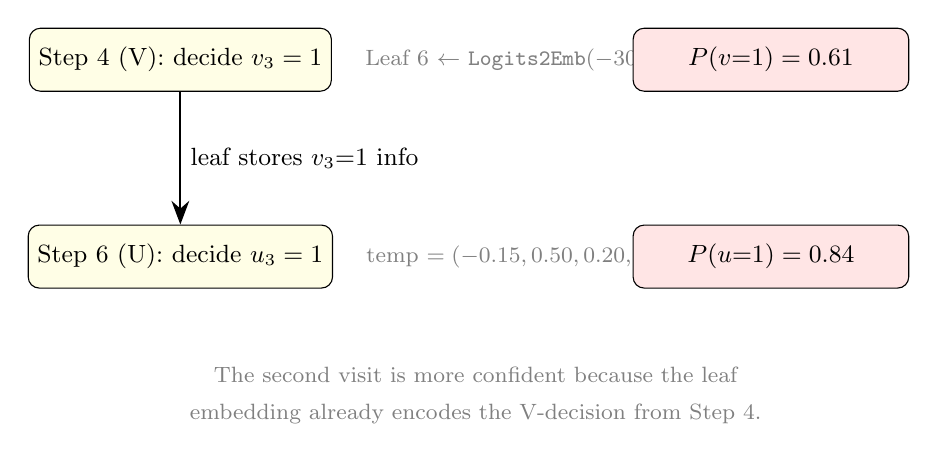
\begin{tikzpicture}[
    box/.style={rectangle, draw, rounded corners, minimum width=3.5cm, minimum height=0.8cm, fill=yellow!10, font=\small},
    arrow/.style={-{Stealth[length=3mm]}, thick},
    note/.style={font=\footnotesize, color=gray}
]
\node[box] (s4) at (0, 0) {Step 4 (V): decide $v_3 = 1$};
\node[box] (s6) at (0, -2.5) {Step 6 (U): decide $u_3 = 1$};

\draw[arrow] (s4) -- (s6) node[midway, right, font=\small] {leaf stores $v_3{=}1$ info};

\node[note, right=0.3cm of s4] {Leaf 6 $\leftarrow$ \texttt{Logits2Emb}$(-30, -0.69, -30, -0.69)$};
\node[note, right=0.3cm of s6] {temp $= (-0.15, 0.50, 0.20, -0.30)$: carries $v_3$ info};

\node[box, fill=red!10] (s4r) at (7.5, 0) {$P(v{=}1) = 0.61$};
\node[box, fill=red!10] (s6r) at (7.5, -2.5) {$P(u{=}1) = 0.84$};

\node[note] at (3.75, -4) {The second visit is more confident because the leaf};
\node[note] at (3.75, -4.5) {embedding already encodes the V-decision from Step 4.};
\end{tikzpicture}
\end{center}

Similarly, the CalcParent operation at Step 4 propagates information \emph{upward} from the left subtree (positions 1--2, fully decided) to enable the right subtree (positions 3--4) to decode with better context.

%=============================================================================
\section{Training vs.\ Inference}
\label{sec:train_vs_infer}
%=============================================================================

\subsection{Teacher Forcing (Training)}

During training, the decoder uses the \emph{true} bit values for leaf updates regardless of its own decisions:
\begin{itemize}[nosep]
\item At Step 3, suppose the network had predicted $\hat{v}_2 = 0$ (incorrect).
\item Under teacher forcing, the leaf update still uses $v_2 = 1$ (true value).
\item This prevents error cascading during training and ensures stable gradients.
\item The loss is always computed against the true target class $c = u_{\text{true}} \cdot 2 + v_{\text{true}}$.
\end{itemize}

\subsection{Inference (No Teacher Forcing)}

During inference, the decoder uses its own hard decisions:
\begin{itemize}[nosep]
\item At each info step, the decision $\hat{b} = \mathbf{1}[P(b{=}1) > P(b{=}0)]$ is used for the leaf update.
\item An error at an early step (e.g., wrong $\hat{v}_2$) propagates to later steps through the leaf embeddings, potentially causing a cascade of errors.
\item Frozen positions are immune: their values are predetermined and always correct.
\end{itemize}

\subsection{Backpropagation}

Gradients flow through the entire computational graph:
\[
\nabla_\theta \mathcal{L} = \frac{1}{|\text{info steps}|} \sum_{t \in \text{info steps}} \nabla_\theta \mathcal{L}_t.
\]
Each loss $\mathcal{L}_t$ depends on:
\begin{enumerate}[nosep]
\item \texttt{Emb2Logits} weights (direct).
\item The combined embedding, which depends on top-down (via \calL/\calR) and bottom-up (via \texttt{Logits2Emb} from prior leaf updates).
\item The root embeddings (\texttt{EmbeddingZ}), reached through chains of \calL, \calR, and \calP{} operations.
\end{enumerate}
All tree operations (\calL, \calR, \calP) are differentiable, so gradients flow from every leaf loss back to the root embeddings and all shared MLP weights.  The GRU-gated \calP{} module is particularly important: its gate learns \emph{how much} of the analytical residual $(\text{left}+\text{right})/2$ to keep versus how much to replace with the learned candidate.

\subsection{Complexity}

Each of the $2N = 8$ steps involves at most $O(\log N) = O(2)$ tree operations, each costing $O(d \cdot h)$ where $h$ is the MLP hidden dimension.  Total: $O(N \log N \cdot d \cdot h)$.  For $N=4$, $d=4$, $h=64$: roughly $4 \times 2 \times 4 \times 64 = 2048$ multiply-add operations per step.

%=============================================================================
\section{Appendix: Partially Deterministic Leaf Embeddings}
\label{sec:leaf_emb}
%=============================================================================

The leaf update rule (\texttt{\_make\_leaf\_emb}) constructs a log-probability vector $\ell \in \R^4$ indexed by $(u,v) \in \{00, 01, 10, 11\}$:

\begin{center}
\begin{tabular}{@{}lll@{}}
\toprule
Known bits & Log-prob vector $\ell$ & Meaning \\
\midrule
Neither & $(\log\tfrac{1}{4},\, \log\tfrac{1}{4},\, \log\tfrac{1}{4},\, \log\tfrac{1}{4})$ & Uniform \\
$u{=}0$ only & $(\log\tfrac{1}{2},\, \log\tfrac{1}{2},\, {-}30,\, {-}30)$ & $u$ fixed, $v$ uniform \\
$u{=}1$ only & $({-}30,\, {-}30,\, \log\tfrac{1}{2},\, \log\tfrac{1}{2})$ & $u$ fixed, $v$ uniform \\
$v{=}0$ only & $(\log\tfrac{1}{2},\, {-}30,\, \log\tfrac{1}{2},\, {-}30)$ & $v$ fixed, $u$ uniform \\
$v{=}1$ only & $({-}30,\, \log\tfrac{1}{2},\, {-}30,\, \log\tfrac{1}{2})$ & $v$ fixed, $u$ uniform \\
$u{=}0, v{=}0$ & $(0,\, {-}30,\, {-}30,\, {-}30)$ & Fully deterministic \\
$u{=}1, v{=}1$ & $({-}30,\, {-}30,\, {-}30,\, 0)$ & Fully deterministic \\
\bottomrule
\end{tabular}
\end{center}

This vector is then transformed by \texttt{Logits2Emb}: $\R^4 \to \R^d$ to produce the new leaf embedding.  Crucially, the leaf stores only the \emph{decision state}, not the accumulated channel information---this prevents double-counting channel evidence on revisit.

\end{document}
